\documentclass{article}
\usepackage{graphicx}
\usepackage{amsmath}
\usepackage{amssymb}
\usepackage{physics}
\usepackage{hyperref}
\usepackage{float}
\usepackage[font=small]{caption}

\begin{document}

\section*{Problem 1: Cantilever Beam under Uniform Load}

\subsection*{Governing Equation}
The Euler-Bernoulli beam equation for deflection \( u(x) \) is given by:
\[
\frac{d^4 u}{dx^4} = -\frac{q}{EI}
\]
where \( E = 200 \times 10^9 \, \text{Pa} \), \( I = 10^{-6} \, \text{m}^4 \), \( q = 10000 \, \text{N/m} \), and \( L = 1 \, \text{m} \).

\subsection*{Boundary Conditions}
\begin{itemize}
    \item \textbf{Fixed end} (\( x = 0 \)):
        \[
        u(0) = 0, \quad \frac{du}{dx}\Big|_{x=0} = 0
        \]
    \item \textbf{Free end} (\( x = L \)):
        \[
        \frac{d^2u}{dx^2}\Big|_{x=L} = 0, \quad \frac{d^3u}{dx^3}\Big|_{x=L} = 0
        \]
\end{itemize}

\subsection*{Analytical Solution}
\[
u_{\text{exact}}(x) = -\frac{q}{EI} \left( \frac{x^4}{24} - \frac{x^3}{6} + \frac{x^2}{4} \right)
\]

\subsection*{PINN Implementation}
\begin{itemize}
    \item \textbf{Architecture}: FNN with 4 layers (1-30-30-30-1)
    \item \textbf{Activation}: \(\tanh\)
    \item \textbf{Optimizer}: Adam (\( \text{lr} = 0.001 \))
    \item \textbf{Loss}: PDE residual + 4 boundary operators
    \item \textbf{Training}: 4000 iterations
\end{itemize}

\begin{figure}[H]
    \centering
    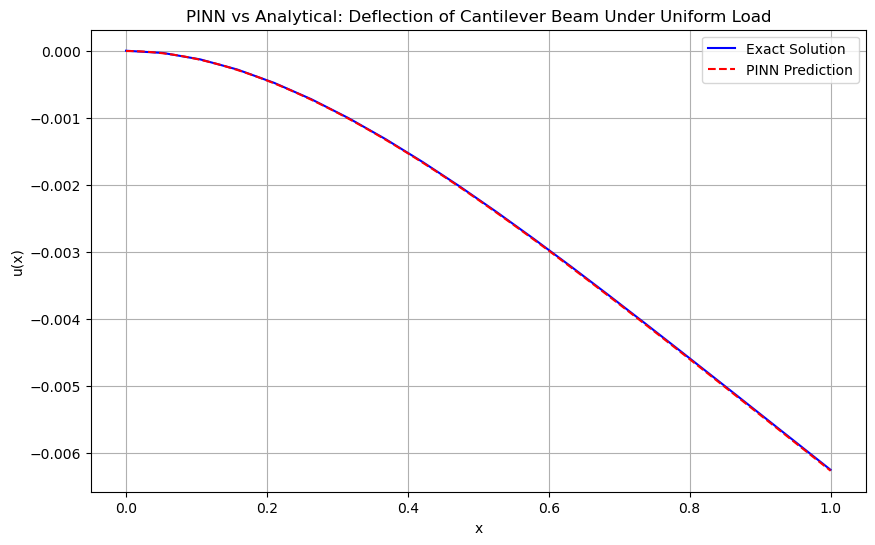
\includegraphics[width=0.8\textwidth]{geom1.png}
    \caption{PINN prediction vs analytical solution for cantilever beam deflection}
    \label{fig:cantilever}
\end{figure}

\end{document}